\chapter{Lavori correlati}
\label{cha:intro}

\section{Convolutional Neural Networks} %fornire conoscenza basilare sulle CNN

Le Convolutional Neural Networks (CNN) rappresentano un pilastro fondamentale nell'ambito della classificazione di immagini mediante algoritmi di machine learning e comprendere il loro funzionamento è essenziale per apprezzarne l'efficacia e per studiarne l'applicabilità nei vari contesti.

% DL

Esse si ispirano al funzionamento del sistema visivo umano, cercando di emulare la capacità del cervello di estrarre automaticamente caratteristiche rilevanti dalle immagini. Una delle proprietà distintive di queste reti è la struttura tipica a strati che svolge un ruolo fondamentale nell'elaborazione di immagini; questa architettura stratificata consente di scomporre il processo di classificazione in una serie di operazioni intermedie, ciascuna con una specifica funzione.

\subsection{Funzionamento}
\label{sec:cnnfunc}
Tipicamente in una CNN si susseguono diversi strati, o \textit{layer}, di operazioni che modificano l'immagine presa in input e la trasformano in rappresentazioni intermedie modificate, che sono difficili da comprendere per l'occhio umano, ma funzionali per l'interpretazione dei layer successivi e del classificatore finale. Le operazioni svolte da ogni strato della rete comprendono la \textit{convoluzione}, applicata tra l'input di uno strato ed il suo filtro (anche detto ``kernel"), ed il \textit{pooling}, ovvero operazioni per ridurre la dimensione delle raffigurazioni intermedie ai vari strati.

Durante la convoluzione, il filtro, solitamente di dimensione $3\times3$ o $5\times5$, scansiona l'immagine di input e calcola la somma del prodotto punto a punto tra i valori dell'input e i pesi del filtro. Il risultato di questa operazione è una rappresentazione, anche detta \textit{feature map}, che evidenzia le caratteristiche rilevanti dell'immagine, come bordi, texture o forme. Le operazioni di pooling hanno invece lo scopo di ridurre la dimensione delle rappresentazioni intermedie ai vari layer, questa funzione viene applicata su una finestra di dimensione predefinita dell'input e consiste nella selezione del valore medio o massimo (rispettivamente average pooling e  max pooling), riducendo la dimensione dell'input e mantenendo le informazioni salienti. Tale processo di riduzione della dimensionalità aiuta a semplificare il modello, diminuendo il numero di parametri e migliorando l'efficienza computazionale. Inoltre, per consentire alle CNN di modellare relazioni complesse, apprendere rappresentazioni gerarchiche e superare la limitazione della linearità intrinseca degli strati di convoluzione, diventa necessario l'utilizzo delle funzioni di attivazione che introducono una non-linearità nel processo di classificazione e aiutano la rete a modellare relazioni complesse nei dati. Queste funzioni trasformano l'output di un neurone in base a una determinata regola e le più utilizzate per il task di classificazione di immagini sono la funzione sigmoide e la ReLU (Rectified Linear Unit) che è particolarmente popolare perché introduce una non-linearità semplice e computazionalmente efficiente, permettendo anche una maggiore velocità di convergenza durante l'apprendimento.

\iffalse
\begin{figure}[ht!]
    \centering
    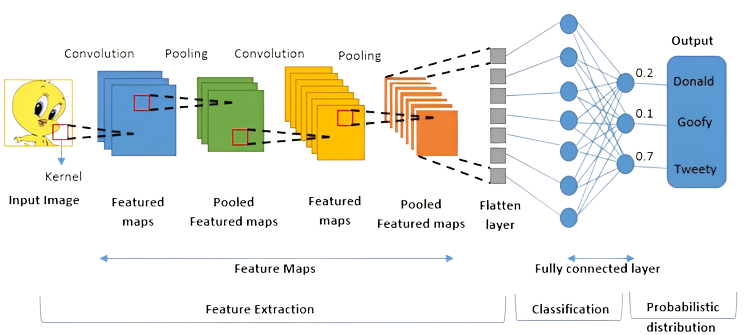
\psfig{file=immagini/cnn.png,width=0.9\textwidth}
    \caption{\textit{Convolutional Neural Network per la classificazione di immagini}.}
    \label{fig:cnn}
\end{figure}
\fi

Attraverso la combinazione di convoluzione e pooling in diversi strati, una CNN è in grado di estrarre progressivamente caratteristiche complesse dall'immagine. I layer iniziali si concentrano su caratteristiche più semplici, come linee e angoli, mentre quelli successivi combinano tali caratteristiche per identificare oggetti più complessi e definire classi specifiche. 
\cite{10.1093}

%softmax
Alla fine degli strati di convoluzione e pooling va posizionato il classificatore, ovvero un layer lineare che prende in input tutte le feature in output dall'ultimo blocco convolutivo e restituisce le probabilità di appartenenza dell'immagine originaria ad ogni classe. \\

Finora abbiamo esaminato il funzionamento e la struttura del modello; tuttavia, è fondamentale anche l'addestramento del modello tramite l'utilizzo di un ampio dataset, che rappresenta un insieme di dati necessario per consentire al modello di apprendere e ottimizzare i suoi pesi.


% Argomenti toccati: caratteristiche dataset, splitting, quali usati e caratteristiche 
\subsection{Dataset} % APPROFONDIRE ARGOMENTO RISOLUZIONE?

Il dataset è una raccolta di dati strutturata che contiene le informazioni necessarie per poter addestrare una rete neurale, in particolare nelle applicazioni di image classification il dataset è costituito da immagini e dalle relative etichette che ne definiscono la classe di appartenenza.

Questi set di dati sono caratterizzati da una vasta diversità e un numero significativo di immagini per ogni classe, fornendo una rappresentazione completa delle categorie di interesse. La qualità del dataset è essenziale: deve essere accurato e bilanciato, con etichette di classe corrette e coerenti. Inoltre, la varietà delle immagini presenti nel dataset deve coprire in modo adeguato le varie categorie e le possibili variazioni all'interno di ogni classe; ciò assicura che il modello sia esposto a una vasta gamma di esempi durante l'addestramento, rendendolo più robusto e garantendone l'efficacia e la capacità di generalizzazione.

% datasplitting holdout method
Per valutare le prestazioni del modello in modo affidabile e imparziale, evitando il rischio di sovradattamento (overfitting) ai dati di addestramento è ampiamente usata la tecnica \textit{data splitting} che consiste nel suddividere il dataset disponibile per l'addestramento in tre diversi raggruppamenti nella maniera più equa possibile; in tal modo si ottengono set di dati indipendenti che possono essere usati in maniera differente durante la fase di addestramento e di valutazione delle performance.
La pratica più comune è quella di suddividere l'insieme rispettivamente in dati di allenamento, o \textit{training set}, che di solito costituiscono l'80\% del dataset originario e sono utilizzati per far imparare al modello i pesi che migliorano l'accuratezza di predizione, dati di validazione, o \textit{validation set}, che ne costituiscono il 10\% e si utilizzano per validare la capacità predittiva e per evitare l'\textit{overfitting}, e dati di test, o \textit{test set}, che ne costituiscono il rimanente 10\% e vengono utilizzati una sola volta per valutare le prestazioni finali del modello ed ottenere una stima accurata delle capacità di generalizzazione della rete su dati mai visti prima, simulando il contesto di applicazione reale.

% MEGLIO ELENCO PUNTATO?
\iffalse
La pratica più comune è quella di suddividere l'insieme rispettivamente in: 
\begin{itemize}
    \item dati di allenamento, o \textit{training set}, che di solito costituiscono l'80\% del dataset originario e sono utilizzati per far imparare al modello i pesi che migliorano l'accuratezza di predizione, minimizzando la discrepanza tra le previsioni del modello e le etichette corrette associate alle immagini di addestramento;
    \item dati di validazione, o \textit{validation set}, che ne costituiscono il 10\% e si utilizzano per monitorare la capacità predittiva del modello su dati mai visti in fase di allenamento e per evitare l'\textit{overfitting};
    \item dati di test, o \textit{test set}, che ne costituiscono il rimanente 10\% e vengono utilizzati una sola volta per valutare le prestazioni finali del modello ed ottenere una stima accurata delle capacità di generalizzazione della rete su dati mai visti prima, simulando il contesto di applicazione reale.
\end{itemize}
\fi

La scelta delle proporzini dei vari set di dati è soggettiva e le opzioni più gettonate per trainig, validation e test set sono 80\%-10\%-10\%, 70\%-15\%-15\% e 60\%-20\%-20\%, ad ogni modo un aspetto cruciale è la suddivisione equa e rappresentativa delle classi e delle variazioni dei dati in ogni set. Ciò garantisce che il modello venga valutato in modo accurato su tutte le categorie e che le sue prestazioni siano generalizzabili. \\

Nel caso studio qui presentato sono stati utilizzati due datasets differenti per mostrare come la scelta del dominio di ricerca influenzi i risultati e poterli quindi confrontare; la scelta è ricaduta su \textit{CIFAR-10} e \textit{CIFAR-100}, due dataset composti da 60mila immagini RGB etichettate di dimensione $32\times32$ pixel che consistono rispettivamente di 10 classi da 6000 immagini ognuna (CIFAR-10) e 100 classi da 600 immagini ciascuna (CIFAR-100), suddivise in set secondo le proporzini 70\%-15\%-15\%, principalmente raffiguranti esseri viventi, mezzi di trasporto e oggetti vari.
\cite{datasets}

% Argomenti toccati: processo training, loss, ottimizzazione, batch size, epoche
\subsection{Training e ottimizzazione}

L'addestramento di una rete neurale per la classificazione di immagini è un passaggio cruciale per insegnare al modello a riconoscere e assegnare correttamente le diverse categorie alle immagini.

Dopo aver suddiviso il dataset secondo le logiche illustrate sopra, e soprattutto dopo aver definito l'architettura di rete da allenare, si passa all'inizializzazione dei parametri del modello da ottimizzare, in particolare per le CNN ci si riferisce ai \textit{pesi} ed ai \textit{bias} utilizzati dagli strati convolutivi. Come già anticipato, infatti, durante una convoluzione le rappresentazioni in input agli strati convolutivi vengono filtrate tramite un prodotto punto a punto tra i valori dei pixel della finestra scorrevole ed i pesi del kernel, i risultati di queste moltpilicazioni vengono poi sommati ed il tutto è addizionato al bias riferito al filtro. Sono proprio questi i parametri che vanno a definire i risultati di classificazione di un modello e l'obiettivo è trovare quella configurazione di pesi e bias dei vari layer che massimizza le performance della rete. È forse inutile affermare che una ricerca esaustiva della configurazione migliore non è una via praticabile data l'enorme quantità di parametri presenti, si rende quindi necessario lo sviluppo di un algoritmo di aggiustamento dei pesi che mira a minimizzare la discrepanza tra le predizioni del classificatore ed i risultati attesi; questo processo prende perciò il nome di \textit{training}.

L'inizializzazione dei parametri consiste quindi nell'assegnare dei pesi predefiniti al modello che verranno in seguito ottimizzati; tale assegnazione può avvenire in diverse modalità, le più comuni sono l'inizializzazione con valori randomici e l'assegnazione secondo criteri che velocizzano la fase di apprendimetno in base alle funzioni di attivazione utilizzate all'interno della rete. Ne è un esempio la tecinca di inzializzazione dei pesi proposta da Kaiming He (ottimizzata per la funzione ReLU) per la quale ogni peso viene inizilizzato secondo una distribuzione normale con media nulla e varianza uguale a $\sqrt{6/N}$, dove \textit{N} è il numero di canali di input del layer convoluzionale.
\cite{1502.01852}

A seguito dell'inizializzazione dei pesi, inizia la fase di allenamento vero e proprio della rete; a questo stadio del processo viene eseguita quella che viene detta \textit{forward propagation}, durante la quale le immagini del trainig set vengono ``propagate" attraverso i vari strati del modello e si ottiene in uscita la predizione di classificazione ottenuta con lo stato presente dei pesi. Questi risultati vengono confrontati con quelli attesi (le etichette delle immagini) e viene calcolata una metrica che ne misura la discrepanza tramite una funzione di perdita, anche detta \textit{loss function}, di cui la più comunemente usata è la Cross-Entropy Loss. L'obiettivo è quello di ridurre al minimo la loss in modo da avere dei risultati di predizione in linea con quelli attesi.

Proprio al fine di minimizzare la perdita, entra in gioco quella che viene detta \textit{backward propagation}, ovvero un algoritmo utilizzato per calcolare il gradiente della funzione di perdita rispetto ai parametri della rete ed esprime il contributo di ciascun peso e bias all'errore totale. Questa operazione avviene utilizzando la regola della catena, o \textit{chain rule}, che applica la derivata parziale in ogni layer per calcolare il contributo della loss rispetto ai parametri di tale strato.

Una volta calcolato il gradiente, l'ottimizzazione viene eseguita utilizzando un algoritmo specifico di aggiornamento dei pesi, i più noti dei quali sono il \textit{gradient descent}, lo \textit{stochastic gradient descent} (SGD) e gli ottimizzatori \textit{Adam} e \textit{Lamb}. Questi processi utilizzano il gradiente calcolato per aggiornare i parametri della rete in modo da ridurre l'errore e migliorare le prestazioni del modello durante l'addestramento.

L'intero processo di ottimizzazione dei parametri dovrebbe essere ripetuto per ogni campione del set di training, in modo che la rete possa imparare da tutte le informazioni a disposizione, e pure per molteplici volte. Tuttavia eseguire l'aggiustamento dei pesi per ognuna delle immagini potrebbe rallentare il processo di addestramento (dato che gli algoritmi del calcolo del gradiente e di ottmizzazione andrebbero ripetuti numerose volte) e potrebbe compromettere la stabilità e la capacità di generalizzazione del modello, visto che la rete si adatterebbe troppo ai singoli esempi che possono essere soggetti a maggiore variazione e rumore.
Per ovviare a questi probelmi è diventata ormai standard la pratica di dividere il set di training in \textit{batch}, ovvero insiemi di immagini (solitamente 64 o 128) che vengono elaborati contemporaneamente prima di eseguire l'aggiornamento dei parametri. Tale metodo consente di ottenere una stima del gradiente più stabile e rappresentativa, poiché il calcolo del gradiente si basa su più esempi e migliora l'efficienza del processo di addestramento.

Un solo passaggio attraverso il set di allenamento non è abbastanza per poter ottenere un modello con buone performance di classificazione, si rende quindi necessario la ripetizione di tutte le azioni precedenti per un certo numero di \textit{epoche} in modo da peremttere alla rete di apprendere dai dati in modo progressivo e poter convergere ad una soluzione ottimale.

\subsection{Valutazione delle prestazioni}

Dopo aver compreso le tecniche più utilizzate per addestrare i modelli di calssificazione di immagini diventa necessario stabilire delle metriche di valutazione delle prestazioni delle reti per essere in grado di confrontarle. Ad ogni epoca infatti lo stato della rete, con i parametri ottimizzati fino a quel momento, può essere salvato al fine di confrontare le sue capacità di generalizzazione con altri modelli di epoche differenti. A tal scopo la metrica di precisione più impiegata è la \textit{top-1 accuracy} che rappresenta la percentuale di volte che il modello ha predetto correttamente la classe come la sua scelta principale. Questa misura di accuratezza di classficazione, per poter essere significativa, è da calcolare sul validation set in maniera tale da avere una metrica di confronto basata su predizioni effettuate su immagini che non hanno influito sull'allenamento della rete.

La fase di confronto di prestazioni sul test di validazione per modelli provenienti da epoche differenti è necessario perchè non sempre addestrare un modello per più epoche comporta avere prestazioni di classificazione migliori su dati mai visti. Questo problema di generalizzazione prende il nome di \textit{overfitting} che si verifica quando un modello di machine learning è eccessivamente adattato ai dati di addestramento e ha scarse capacità di predizione su nuovi esempi. 

Per avere una stima delle reali performance di classificazione della rete si valuta il modello scelto dal confronto precedente sul set di immagini di test che fornisce una stima imparziale delle prestazioni della rete su dati che non ha mai visto prima, consentendo di valutare la capacità di generalizzazione del modello.

\iffalse
-----------------------
cose da dire:
\begin{itemize}
    \item Funzionamento delle CNN: panoramica del funzionamento delle CNN, spiegare  convoluzione, pooling e struttura a strati. Descrivere l'importanza dei pesi dei neuroni e delle funzioni di attivazione nel processo di apprendimento delle CNN.
    \item Pre-elaborazione dei dati: Illustrare l'importanza della pre-elaborazione dei dati per la classificazione di immagini, inclusi normalizzazione dei pixel,  riduzione del rumore e gestione delle dimensioni delle immagini.
    \item Addestramento e ottimizzazione dei modelli: Spiegare il processo di addestramento dei modelli, incluso l'utilizzo di dataset, funzioni di costo e l'ottimizzazione dei parametri.
    \item Valutazione delle prestazioni dei modelli: Descrivere le metriche comuni utilizzate per valutare le prestazioni, come accuratezza, precisione, richiamo (f1 score)
\end{itemize}
\fi


%1 mobile net: alpha, 
%2 efficientnet: compound scaling
    % compound sclaing con efficient net 
%3 mcu net: blocchi convoluzionali, inference engine ottimizzato

\section{Architetture di deep learning per l'edge computing}

Negli ultimi anni c'è stata una crescente necessità di spostare le architetture di deep learning come le Convolutional Neural Networks su dispositivi di edge computing; esigenza che è emersa a causa di diversi fattori spiegati in precedenza, tra cui il bisogno di ridurre la latenza e la larghezza di banda richiesta e la necessità di elaborare i dati in tempo reale.

Per soddisfare questa richiesta, sono state sviluppate architetture di tinyML come MobileNets, EfficientNet e MCUNet progettate appositamente per essere efficienti in termini di risorse computazionali, memoria e consumo energetico, al fine di poter essere eseguite su dispositivi con capacità limitate, come smartphone, dispositivi IoT e microcontrollori.
\cite{MobileNets}
\cite{EfficientNet}
\cite{MCUNet}

\subsection{MobileNets}
\label{sec:mobilenets}

MobileNets rappresenta una famiglia di CNN ampiamente utilizzata per applicazioni di computer vision, come la classificazione di immagini, per dispositivi mobili ed embedded. 

Una delle caratteristiche distintive di MobileNets è la sua struttura innovativa che permette di ottenere modelli efficienti e leggeri e si basa sull'idea di convoluzioni depthwise separabili, che scindono il classico processo di convoluzione in due fasi distinte: la \textit{depthwise convolution} e la \textit{pointwise convolution}. 

Le convoluzioni tradizionali applicano un filtro completo a tutti i canali di input, ciò significa che per ogni filtro vengono calcolate le convoluzioni su tutti i canali di input, generando un numero significativo di operazioni. D'altra parte, le convoluzioni depthwise separabili dividono il processo della convoluzione sui canali (\textit{depthwise}) da quella sui singoli pixel (\textit{pointwise}), in modo da ridurre l'onere computazionale. La convoluzione depthwise applica un singolo filtro a ciascun canale di input, riducendo il numero di parametri e operazioni computazionali; successivamente, la convoluzione pointwise combina linearmente i canali di output della convoluzione depthwise, generando un set di rappresentazioni finali (feature maps).

\begin{figure}[ht!]
    \centering
    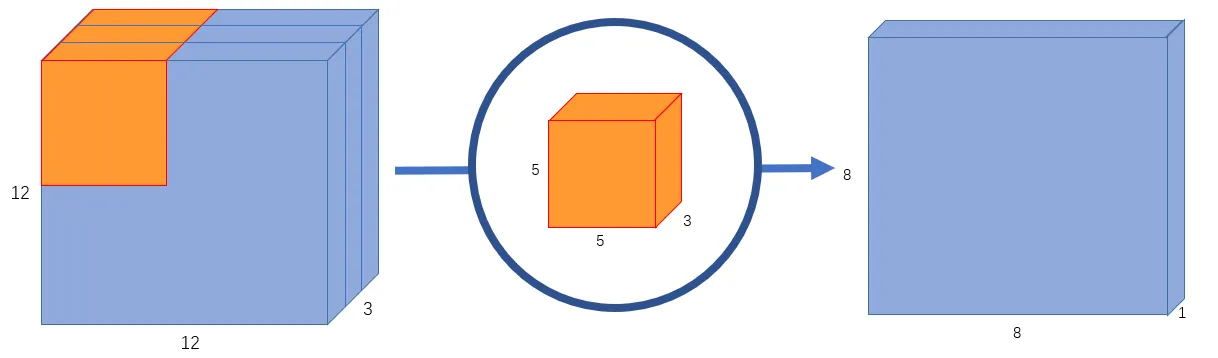
\psfig{file=immagini/traditional_conv.png,width=0.8\textwidth}
    \caption{\textit{Convoluzione tradizionale}. In questo caso l'immagine originaria ha risoluzione $12\times12$ ed è composta da 3 canali (come nel caso di una foto RGB). Un filtro convolutivo completo si estende su tutti i canali dell'immagine e genera in uscita una rappresentazione ad un singolo canale con risoluzione minore. Se si volesse avere come output una feature map composta da \textit{N} canali (come spesso succede nelle CNN), bisognerebbe quindi avere \textit{N} filtri convolutivi ed eseguire \textit{N} convoluzioni. Nel caso qui rappresentato l'intero processo richiederebbe $4800\times N$ moltiplicazioni.}
\end{figure}

\begin{figure}[ht!]
    \centering
    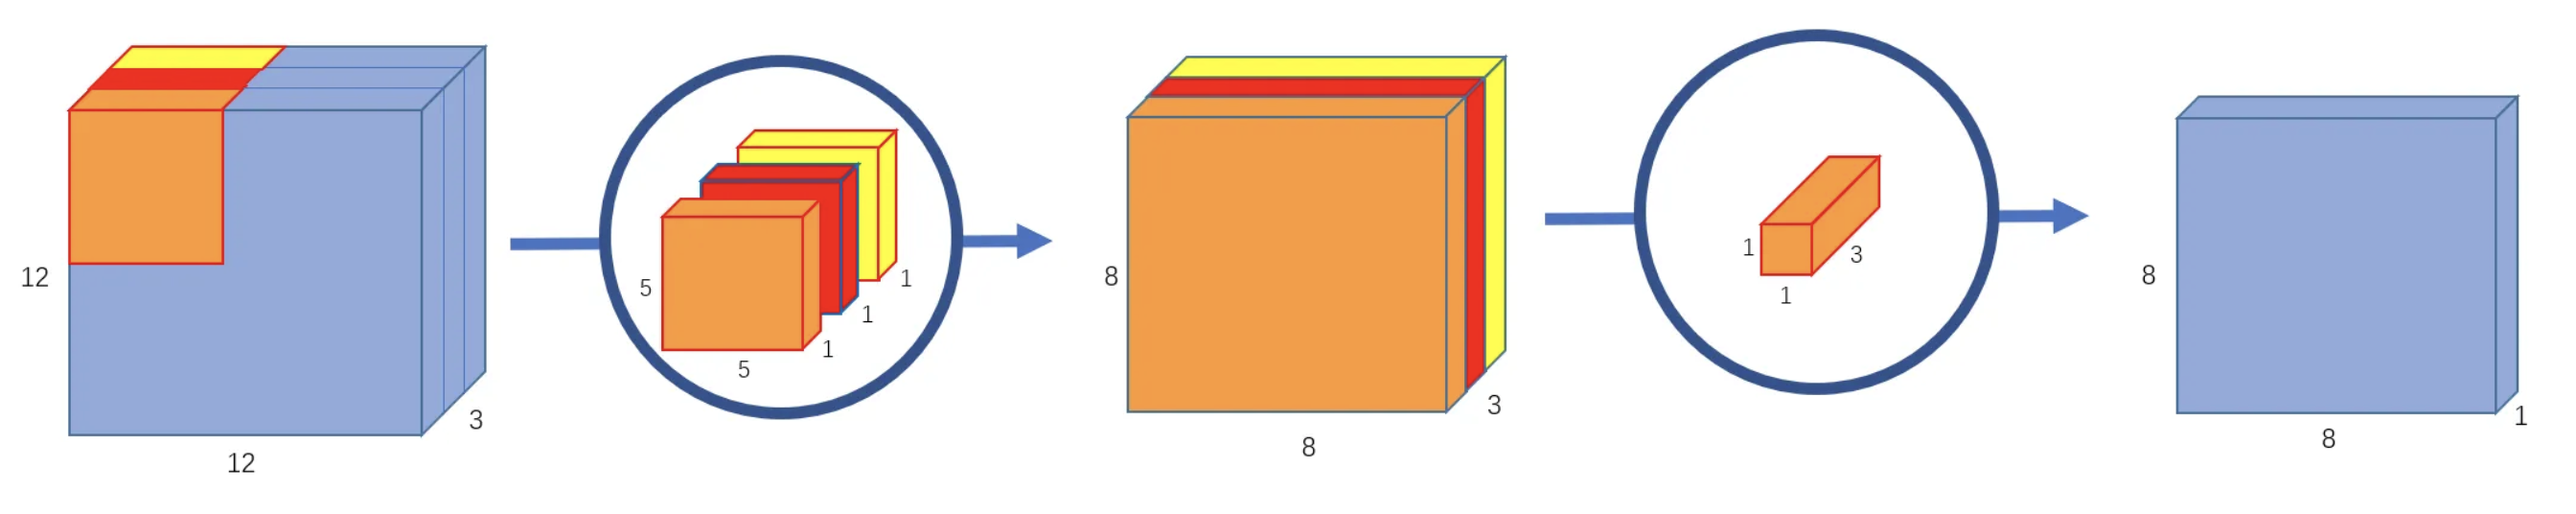
\psfig{file=immagini/depthwise_separable_conv.png,width=1.0\textwidth}
    \caption{\textit{Convoluzione depthwise separabile}. La stessa immagine di partenza viene prima fatta passare attraverso una convoluzione sui canali (depthwise) e si ottiene una rappresentazione intermedia ancora divisa secondo il numero di canali originario; per ottenere in output una rappresentazione ad un solo canale si esgue la convoluzione spaziale sui pixel dell'immagine (pointwise). Al fine di estrarre una feature map composta da \textit{N} canali, bisognerebbe soltanto avere \textit{N} filtri convolutivi pointwise ed eseguire \textit{N} convoluzioni pointwise, che sono ovviamente più leggere ed efficienti. Nel caso qui rappresentato l'intero processo richiederebbe un totale di $4800 + 192\times N$ moltiplicazioni, che nei casi di applicazione reali si traduce in un guadagno enorme nell'efficienza del modello.}
\end{figure}

Un altro aspetto innovativo delle MobileNets è l'introduzione dei fattori di scala che consentono di adattare le dimensioni e la complessità della rete in base a delle specifiche esigenze di risorse computazionali. 

I due fattori di scaling presentati in questo tipo di architettura sono dei moltiplicatori che regolano rispettivamente il numero di canali in input e in output ad ogni layer ($\alpha$  \textit{width multiplier}) e la risoluzione in ingresso delle immagini ($\rho$  \textit{resolution multiplier}).

Sebbene il fattore di regolazione della risoluzione non sia una colonna portante di questo tipo di reti, in quanto lo si può impostare implicitamente modificando la risoluzione delle immagini in ingresso al modello, esso aiuta a comprendere come la modifica delle dimensioni delle immagini influenzi il numero di operazioni eseguite dal modello. Scegliendo infatti valori del moltiplicatore $\rho$ appartenenti all'intervallo $(0, 1]$ il  costo computazionale si riduce di $\rho^{2}$ dato che il numero di operazioni di convoluzione necessarie per analizzare un immagine aumenta quadraticamente rispetto alle sue dimensioni.

Il fattore di regolazione dei canali ha invece il ruolo di assottigliare la rete uniformemente ad ogni strato; scegliendo infatti valori di $\alpha$ nell'intervallo $(0, 1]$ si va a modificare il numero di canali in ingresso \textit{M} ed in uscita \textit{N} da ogni layer convolutivo rispettivamente in $\alpha M$ e $\alpha N$. Il \textit{width multiplier} ha quindi l'effetto di ridurre il costo delle convoluzioni depthwise separabili ed il numero di parametri della rete di $\alpha^{2}$, ottenendo così un modello più leggero. 

%Ovviamente non bisogna dimenticare che bilanciare il consumo di risorse di un modello può avere un impatto sull'accuratezza di classificazione, è pertanto necessario gestire attentamente il tradeoff tra efficienza e precisione per ottenere il miglior compromesso tra risorse e prestazioni.

Ovviamente non bisogna dimenticare che bilanciare il consumo di risorse di un modello può avere un impatto sull'accuratezza di predizione della rete, utilizzando ad esempio un fattore $\alpha$ molto piccolo è possibile ottenere una MobileNet leggera e con pochi consumi, ideale per dispositivi mobili con risorse limitate, ma con scarse prestazioni di classificazione. È pertanto necessario gestire attentamente il tradeoff tra efficienza e precisione per ottenere il miglior compromesso tra risorse e prestazioni.

\subsection{EfficientNet ed il compound scaling}

Un'altra tipologia di architettura che si propone di implementare reti convoluzionali efficienti su dispositivi embedded e mobili è EfficientNet.

Fino all'introduzione di questa famiglia di reti, tra le applicazioni di tinyML che intendevano adattare modelli di CNN a dispositivi con risorse limitate, era comune applicare fattori di scala su una sola delle dimensioni caratteristiche del modello; ad esempio le ResNet \cite{ResNet} possono esserre scalate modificando il numero di strati della rete, mentre le MobileNets possono essere ridimiensionate in base al numero di canali.
L'idea principale dietro EfficientNet è invece quella di trovare un equilibrio tra la profondità (\textit{depth}), la larghezza (\textit{width}) e la risoluzione dell'immagine (\textit{image size}) di input della rete, dato che studi empirici dimostrano che il bilanciamento congiunto di tali fattori è cruciale per ottenere buone performance. 

Per ottenere ciò, EfficientNet utilizza una tecnica chiamata \textit{Compound Scaling}, che regola in modo proporzionale il numero di layer, di canali e la dimensioni delle immagini in input della rete. Ciò significa che all'aumentare della profondità del modello, aumenta anche la larghezza e la risoluzione dell'immagine di input, mantenendo un equilibrio tra queste tre dimensioni chiave.

%\newpage

\subsubsection{Compound scaling}

Ragionando puramente a livello intuitivo, il metodo del compound scaling risulta efficace perchè all'aumentare delle dimensioni delle immagini in input al modello, diventa necessario l'utilizzo di più canali nelle rappresentazioni intermedie per catturare pattern più dettagliati ed un numero maggiore di layer convoluzionali per aumentare la capacità percettiva della rete. Già altri studi avevano evidenziato l'esistenza di una certa correlazione tra la larghezza e la profondità di una CNN, ma questa tecnica di scaling qunatifica empiricamente la relazione tra le tre dimensioni del modello.

\begin{figure}[ht!]
    \centering
    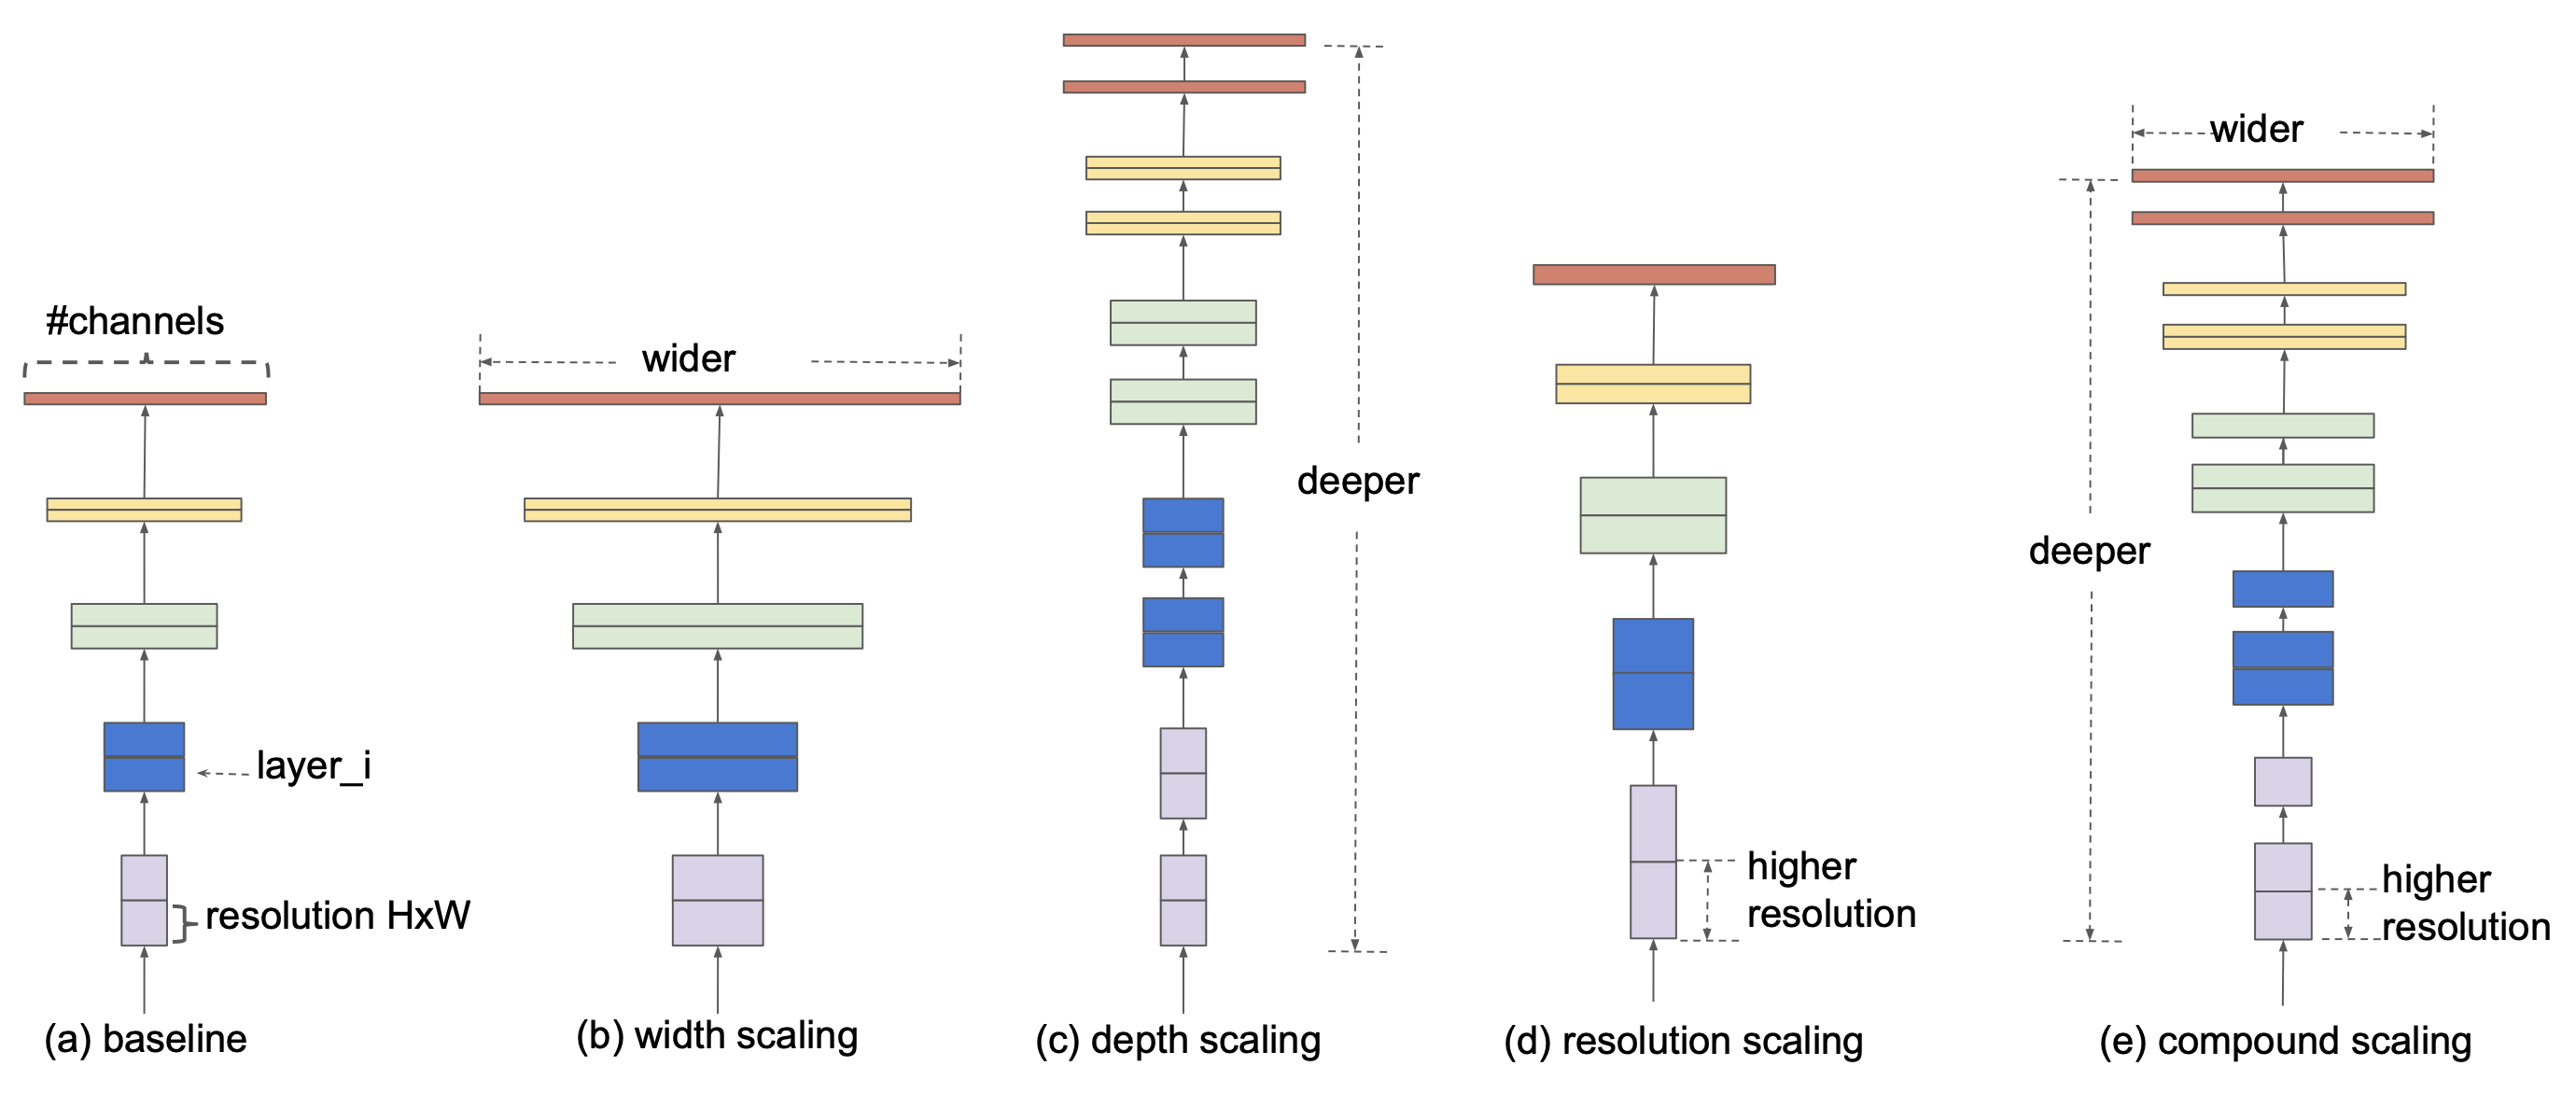
\psfig{file=immagini/efficientnet.png,width=1.0\textwidth}
    \caption{\textit{Scaling delle Convolutional Neural Newtworks}. (a) è la rete di riferimento; (b)-(d) mostrano i metodi convenzionali di scaling in cui viene scalata solo una dimensione tra larghezza, profondità e risoluzione dell'immagine; (e) mostra il metodo di compound scaling che ridimensiona uniformemente tutte e tre le dimensioni con un rapporto fisso.}
    \label{fig:scaling}
\end{figure}

Come mostrato nella figura \ref{fig:scaling} la tecnica del compound scaling mira a conciliare tre diversi metodi di ridimensionamento di una rete neurale convoluzionale, che sono il \textit{width}, \textit{depth} e \textit{resolution scaling}. 
Per lo scaling di queste dimensioni della rete l'architettura di EfficientNet propone tre differenti coefficienti di scala, o \textit{iperparametri}, per regolare le caratteristiche della rete; tali fattori sono:
\begin{itemize}
    \item $\alpha^{\phi}$: regola la profondità (depth) della rete cambiando il numero di layer presenti in modo da poter catturare rappresentazioni più complese;
    \item $\beta^{\phi}$: modifica la larghezza (width) del modello tramite il numero di canali in ingresso e in uscita di ogni layer in maniera analoga al funzionamento del width multiplier presentato nella sezione \ref{sec:mobilenets};
    \item $\gamma^{\phi}$: regola le dimensioni (image resolution) delle immagini in ingresso alla rete secondo le stesse logiche del resolution multiplier della sezione \ref{sec:mobilenets}.
\end{itemize}

L'idea innovativa avanzata dal metodo del compund scaling è l'introduzione del parametro $\phi$ e l'impostazioni degli iperparametri in modo che:
\begin{equation}
  \centering
  \alpha \cdot \beta^{2} \cdot \gamma^{2} \approx 2 \qquad \alpha \ge 1, \, \beta \ge 1, \, \gamma \ge 1
  \label{eq:formula}
\end{equation}

Le combinazioni di questi fattori sono potenzialmente infinite ma possono essere facilmente determinati con una griglia di ricerca basilare; il coefficiente di composizione $\phi$ invece è specificato dall'utente e regola le risorse necessarie per il funzionamento del modello. Dato che in una rete convoluzionale il numero di operazioni eseguite (paragonabile al consumo di potenza) è proporzionale a $depth, width^{2}, resolution^{2}$ del modello e che è stata impostata la relazione \ref{eq:formula} tra gli iperparametri, ne consegue che scegliendo arbitrariamente un valore di $\phi$, il numero di operazioni viene incrementato approssimativamente di $2^{\phi}$.

L'effetto combinato di questi fattori di scala permette quindi ad EfficientNet di raggiungere un giusto equilibrio tra potenza di calcolo, numero di parametri e prestazioni di classificazione.

\subsection{MCUNet ed il tinyNAS}

MCUNet rappresenta un'innovativa architettura progettata per affrontare il complesso problema di portare le convolutional neural networks su piccoli dispositivi per l'Internet of Things e su microcontrollori (MCU, microcontroller units) a basse risorse; questa risulta essere una sifda molto complicata dato che i budget di memoria per queste piattaforme è di 2-3 ordini di grandezza inferiore rispetto a quanto disponibile per i dispositivi mobili.
Queste tipologie di reti si basano su tecniche avanzate di ottimizzazione e compressione del modello, al fine di ridurre drasticamente la complessità computazionale e la quantità di memoria richiesta; tali metodi comprendono la separazione delle operazioni di calcolo e memorizzazione e l'utilizzo della quantizzazione a bassa precisione per rispettare i vincoli di risorse del microcontrollore.

L'\textit{inference engine} di MCUNet è un framework operativo progettato appositamente per massimizzare l'efficienza computazionale e ridurre al minimo l'accesso alla memoria. 
%La separazione delle operazioni di calcolo e memorizzazione in MCUNet è una tecnica progettata per massimizzare l'efficienza computazionale e ridurre al minimo l'accesso alla memoria. 
Invece di eseguire tutte le operazioni di calcolo e memorizzazione in modo sequenziale, MCUNet separa queste due fasi e le esegue in modo asincrono: durante la fase di calcolo, vengono eseguite le operazioni di convoluzione e moltiplicazione con i pesi del modello, che richiedono un'alta potenza computazionale ma un accesso limitato alla memoria;
nella fase di memorizzazione, i risultati delle operazioni di calcolo vengono temporaneamente archiviati in una cache o in registri a bassa latenza. 

Questo permette di ridurre al minimo l'accesso alla memoria principale, che è più lento e richiede più energia. Inoltre, la cache o i registri possono essere organizzati in modo ottimale per sfruttare le caratteristiche del modello e ridurre al minimo il trasferimento di dati tra la memoria principale e l'unità di calcolo.
Grazie a questa separazione delle operazioni di calcolo e memorizzazione, MCUNet riesce a minimizzare l'\textit{overhead} associato all'accesso alla memoria, massimizzando così l'efficienza computazionale.

Per quanto riguarda i limiti di memoria, questa architettura utilizza tecniche di quantizzazione a bassa precisione per ridurre la complessità del modello; tali metodi comportano la rappresentazione dei pesi e degli output intermedi del modello con una precisione inferiore rispetto allo standard di 32 bit.
In particolare MCUNet utilizza la rappresentazione a 8 bit e ciò che permette di ridurre drasticamente lo spazio occupato dalla rete ed il costo computazionale necessario, dato che tali operazioni a precisione inferiore richiedono un dispendio di risorse significativamente inferiore.
Questa riduzione della precisione può comportare una certa perdita di precisione nel modello, tuttavia spesso tale riduzione è accettabile e compensata dai notevoli vantaggi in termini di riduzione di consumo di risorse del modello. 

Con queste accortezze MCUNet ottiene ottime performance di classificazione, in partcicolare raggiunge una \textit{top-1 accuracy} del 70.7\% valutata su ImageNet (un dataset contente oltre 1 milione di immagini divise tra 1000 classi, spesso preso come riferimento per le prestazioni di modelli di classificazione di immagini) sul microcontrollore STM32H743. Altre reti con caratteristiche simili avevano raggiunto risultati affini, MobileNetV2-0.75 ad esempio arriva ad un'accuratezza del 69.8\%, tuttavia MCUNet lo fa riducendo l'utilizzo di memoria SRAM di un fattore $3.5\times$ e l'utilizzo della Flash di un fattore $5.7\times$ per adattarsi meglio ai dispositivi \textit{tiny}.

\subsubsection{Neural Architecture Search (NAS) e tinyNAS}

La ricerca di architetture neurali ottimali per applicazioni specifiche è un ambito di studio noto come Neural Architecture Search (NAS). A differenza dei metodi tradizionali che richiedono un progetto manuale da parte di esperti, NAS utilizza algoritmi di ricerca automatica per esplorare un vasto spazio di possibili architetture, sfruttando tecniche di ottimizzazione e strategie di ricerca per individuare configurazioni neurali ottimali, consentendo di raggiungere risultati di elevata qualità in maniera più efficiente.

Il tinyNAS comprende invece metodi di ricerca di modelli di tinyML concentrandosi sul perfezionamento delle reti per adattarsi alle restrizioni di memoria e potenza computazionale dei dispositivi embedded.
In particolare in MCUNet la fase di indagine inizia con la definizione di uno spazio di ricerca, che rappresenta l'insieme delle possibili configurazioni dell'architettura neurale; questo \textit{search space} viene definito tramite due diversi paramteri: la dimensione delle immagini di input, che varia su 12 diverse risluzioni, ed il width multiplier, che assume 9 diversi valori compresi nell'intervallo $[0.1, 1]$. In totale si ottengono quindi 108 diversi spazi di ricerca che vengono valutati tramite lo studio dei \textit{FLOPs} (Floating point Operations Per Second) corrispondenti; questa analisi si basa infatti sull'assunzione che, per la stessa famiglia di modelli, le necessità computazionali siano positivamente correlate con le performance della rete.

\section{Linear Probes}
\label{sec:probes}

I modelli di Deep Learning, come le Convolutional Neural Networks, possono essere estremamente complessi, con milioni di parametri e strati di calcolo interconnessi. Questa complessità può rendere difficile per le persone comprendere come il modello giunge a un determinato risultato.

Per questo motivo uno dei trend crescenti nel campo del machine learning è quello dell'\textit{interpretabilità} dei modelli; con ciò ci si riferisce appunto alla capacità di comprendere e spiegare il funzionamento e le decisioni prese da una rete neurale. Questo concetto di interpretabilità sta diventando sempre più rilevante nel campo della ricerca informatica sia per motivi etico/normativi (in alcuni settori come quello della sanità o della finanza infatti è richiesto che i modelli siano comprensibili e spiegabili per potersi conformare a regolamentazioni specifiche), sia per motivi di analisi ed ottmizzazione (il funzionamento completo e profondo di una rete spesso non è chiaro neanche agli sviluppatori, per questo motivo riuscire ad interpretare un modello può tornare utile per il suo miglioramento).

Una delle tecniche volte a questo tipo di studio è quella del \textit{Linear Probing} \cite{linearprobes} che consisite nell'analizzare il ruolo dei layer convolutivi intermedi all'interno di una CNN tramite dei classificatori lineari, anche detti \textit{probes}, che vanno a valutare prestazioni di un modello a differenti profondità della rete. Le novità introdotte con questa metodologia hanno implicazioni sicuramente interessanti per quanto riguarda il tema dell'interpretabilità e di analisi delle performance dei modelli di ML, in particolare si nota come il livello di separabilità lineare delle feature in output dai vari strati convolutivi aumenta monotonicamente raggiugngendo layer più profondi della rete.

\subsubsection{Funzionamento delle Linear Probes}

Dato che l'obiettivo di questo tipo di analisi è lo studio delle performance di una determinato modello di convolutional neural network per la classificazione di immagini, è necessario essere già in possesso una rete neurale allenata a tale scopo. Tipicamente, a meno di dettagli implementativi, una CNN per l'image classification segue il funzionamento descritto nella sezione \ref{sec:cnnfunc} ed è composta da diversi layer convolutivi, seguiti da operazioni di pooling, dediti all'estrazione delle feature e da uno strato classificatore finale, che raccoglie tutte le informazioni ricavate e restituisce una distribuzione di probabilità delle classi di appartenenza dell'immagine, come mostrato dallo schema in figura \ref{fig:cnn}. 

\begin{figure}[ht!]
    \centering
    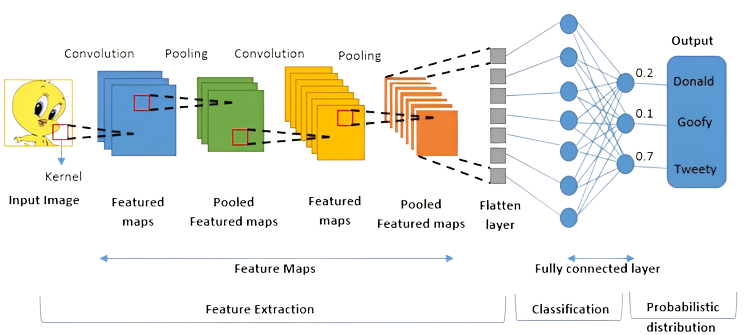
\psfig{file=immagini/cnn.png,width=0.9\textwidth}
    \caption{\textit{Convolutional Neural Network per la classificazione di immagini}.}
    \label{fig:cnn}
\end{figure}

Il principio dietro alla tipologia di esame delle linear probes è quindi quello di posizionare in mezzo ai diversi strati della rete dei classificatori lineari (o probes), che hanno la stessa funzionalità di quello locato al termine del modello, allenarli singolarmente con le sole informazioni estratte fino alla profondità in cui sono disposti ed analizzare le loro prestazioni di classificazione. Queste probes, oltre che per la loro disposizione, differiscono in dimensionalità, ogni strato convolutivo infatti restituisce una rappresentazione (o feature map) caratterizzata da un certo numero di canali e da una precisa dimensione che differsicono dagli output successivi; ogni probe deve essere quindi dimensionata in modo da poter ricevere in ingresso le feature in uscita dal layer ad essa precedente; ogni probe differirà dalle altre anche per i valori (ed il numero) dei pesi, ma avranno tutte la stessa dimensione di output, ovvero il numero di classi, dato che essendo classificatori vengono allenate con le etichette di classe delle immagini provenienti dallo stesso dataset di training della rete.

\subsubsection{Analisi e valutazione}

A seguito della fase di addestramento delle diverse probes si possono confrontare i risultati di classificazione per comprendere al meglio il funzionamento interno della rete. Per fare ciò la metrica più significativa da analizzare è la \textit{loss} che descrive la discrepanza tra le predizioni effettuate dai classificatori e le reali etichette di classe delle immagini. Se il modello di CNN è stato architettato in maniera efficace ci si aspetta un andamento decrescente della metrica di perdita rispetto alla profonidtà del classificatore come illustrato in figura \ref{fig:probe}.

Questa tecnica del Linear Probing aiuta quindi a comprendere il comportamento di una rete neurale convoluzionale per la classificazione di immagini, mostrando come ogni layer della CNN contribuisce alle performance finali del modello, incremenentando il livello di separabilità lineare delle feature man mano che si raggiungono strati più profondi della rete. Tale metodo si dimostra inoltre molto utile per debuggare modelli durante le fasi di sviluppo o per avere concezione del progresso della fase di training in una rete ben strutturata. 

\begin{figure}[ht!]
    \centering
    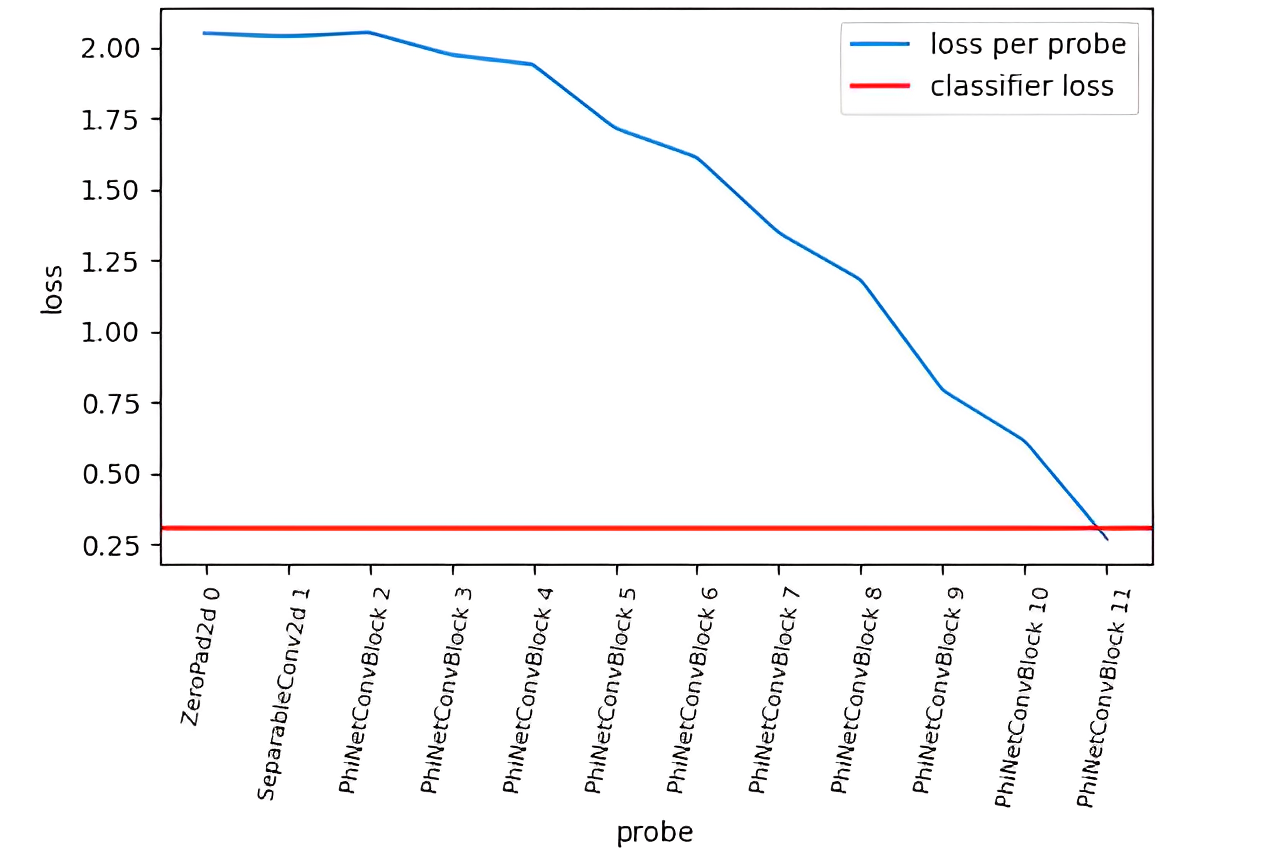
\psfig{file=immagini/loss_per_probe.png,width=0.5\textwidth}
    \caption{\textit{Loss per probe}. Un valore inferiore della funzione di loss corrisponde ad una maggiore accurateza di classificazione.}
    \label{fig:probe}
\end{figure}

\section{Chinchilla scaling law}
\label{sec:chinchilla}

Nel complesso ambito delle architetture di machine e deep learning, i processi di addestramento e valutazione di reti neurali possono richiedere un notevole dispendio di risorse computazionali e temporali, soprattutto quando si considerano differenti configurazioni di un modello. Sorge quindi la necessità di capire se e come sia possibile 
stimare le performance di una rete senza il bisogno di allenarla, ma solamente conoscendo la sua complessità ed i metodi che si intendono utilizzare durante la fase di training. 

A tal proposito nel marzo 2022 è stata proposta da un articolo di DeepMind \cite{chinchilla} una legge di scalabilità che mira a legare le prestazioni di un modello di linguaggio naturale (quelli che vengono definiti Large Language Models, LLM, come ChatGPT) con le sue dimensioni e con la quantità di dati utilizzata durante la fase di addestramento.
In particolare questa legge, che prende il nome di ``Chinchilla scaling law" mette in relazione la metrica di \textit{loss} con la dimensione del modello, in termini di numero di parametri totali (\textit{N}), e della quantità di dati di training, come numero di tokens (\textit{D}), tramite una funzione iperbolica così definita:

\begin{equation}
    \centering
    Loss(N,D) = \frac{A}{N^{\alpha}} + \frac{B}{D^{\beta}} + E
\end{equation}

con $A$ e $B$ che regolano rispettivamente il peso della complessità della rete e dei dati a dispozione sulla loss del modello ed $E$ che misura la perdita per un processo generativo di testo ideale e dovrebbe corrispondere all'entropia del testo naturale.

È interessante notare come la configurazione di parametri (A, B, E, $\alpha$, $\beta$) che meglio approssima l'andamento dei risultati attaulamente in possesso mostri che i ritorni derivanti dall'aumento delle dimensioni del modello sono scarsi, mentre quelli provenienti dall'aumento della quantità di dati sono elevati. Ciò sta a significare che, nel campo dei \textit{transformers} (ovvero un tipo di architettura di rete neurale efficiente per il trattamento di dati sequenziali, come il caso del linguaggio naturale),  al momento il limite principale per le prestazioni dei modelli di linguaggio è la quantità di dati disponibili e, qualora se ne disponga di una quantità sufficiente, non c'è motivo di addestrare modelli con enormi dimensioni (in questo ambito si parla di reti con oltre 500 miliardi di parametri dato che il compito è molto complesso).

Ovviamente le architetture dei transformers generativi per il linguaggio naturale hanno poco in comune con le reti neurali convoluzionali, sia per il compito che per la struttura di rete utilizata, ma la \textit{Chinchilla scaling law} offre buoni spunti per relazionare le performance di un modello di classificazione di immagini con la sua complessità.


%no phinet, (

%1 mobile net: alpha, 
%2 efficientnet: compound )
%compound sclaing con efficient net 
%3 mcu net: blocchi vconvoluzionali, inference engine ottimizzato

%tiny nas in mcunet
%nas 

%linear probes

%chinchilla 
%inizio transormers 
%noi reti convoluxionali 
%fatta con loss, far vedere relazione loss acc
